\newcommand{\textcyrillic}{}
\chapter{Attributive constructions}
\section{Introduction}
\label{bkm:Ref262028996}

One area of grammar where Scandinavian languages show some well-known peculiarities is in the expression of definite noun phrases which contain preposed attributes. In all varieties of Central Scandinavian, a preposed definite article is employed in such noun phrases; however, whereas this article in Danish has a complementary distribution to the ordinary suffixed article, as illustrated by \textstyleLinguisticExample{det store hus} ‘the big house’ (as opposed to \textstyleLinguisticExample{huset} ‘the house’), Swedish (and also normally Norwegian) uses both articles, as in \textstyleLinguisticExample{det stora huset} ‘the big house’. However, in northern Scandinavia, there is a radically different way of combining an adjective and a noun: the normal translation of ‘the big house’ would be something like \textstyleLinguisticExample{stor-hus-et} ‘big-house-{\def}’, where the adjective is incorporated into the noun and there is no preposed article. In this chapter, I shall discuss this construction and a number of additional variations on the general theme that contribute to a quite variegated picture. However, one challenge in doing so is the tight interaction of several different parameters with different histories and geographical distribution. Another problem is the low frequency of adjectival modifiers in definite noun phrases (noted by \citet{Thompson1988}). In the corpus \textit{Samtal i Göteborg }(\citet{Löfström1988}), comprising half a million words of spoken Swedish – corresponding to 1250 printed pages, there were only 253 examples of the pattern

\ea 
\gl den/det/dom Adj-e/a N-{\def}
\z 

that is, the standard form of such NPs in Swedish. (Comparatives and superlatives were excluded from this count.) This is equivalent to about once in ten minutes of conversation, or once in five printed pages. In addition, it turns out that a few adjectival lexemes had a rather dominant place among those examples: about 40 per cent consisted of tokens of the four adjectives \textstyleLinguisticExample{stor }‘big’, \textstyleLinguisticExample{liten} ‘small’, \textstyleLinguisticExample{gammal} ‘old’, \textstyleLinguisticExample{ny} ‘new’. It is probably no accident that these items are among the cross-linguistically prototypical adjectives in the sense that they show up in practically every language that has a separate class of adjectives.\footnote{\label{fnt:ftn36} According to \citet{Dixon1977}, the adjectives that occur most frequently across languages are ‘large’, ‘small’, ‘long’, ‘short’, ‘new’, ‘old’, ‘good’, ‘bad’, ‘black’, ‘white’.} In written dialect texts, which are either direct renderings of spoken language or else tend to be close to spoken language in form, the corresponding patterns also show up very sparingly.

\section{Definite marking in attributive constructions: The typological perspective}

As it turns out, it is quite common cross-linguistically for attributive constructions to show some peculiarities with respect to definiteness marking. Thus, we find languages in which definiteness is only marked when a noun phrase contains a modifier, as in Latvian which has suffixed definite articles on adjectives, although it does not otherwise use definite marking, as illustrated by the following examples. 

\ea\label{}
\langinfo{Latvian}{}{}\\
\ea {
\gll liel-a  m\=aja\\
big-F.{\nom}.{\sg}  house\\
\glt ‘a big house’
}

\ex {
\gll liel-\=a  m\=aja\\
big-F.{\nom}.{\sg}.{\def}  house\\
\glt ‘the big house’
}
\z 
\z 

In another pattern, an article that usually sits on the noun shows up on the adjective in an attributive construction, as exemplified by Amharic:

\ea\label{}
\langinfo{Amharic }{}{}\\
\ea {
\gll bet-u\\
house-{\def}\\
\glt ‘the house’
}

\ex {
\gll t\textcyrillic{?ll?q-}u  bet\\
big-{\def}  house\\
\glt ‘the big house’
}
\z 
\z 

Finally, the phenomenon of double articles is by no means restricted to Scandinavian. Consider, for example, Standard Arabic, in which the noun and the adjective each take the identical article \textstyleLinguisticExample{al}:

\ea\label{}
\langinfo{Standard Arabic}{}{}\\
\ea {
\gll al\textbf{{}-}bayt\\
{\def}-house\\
\glt ‘the house’
}

\ex {
\gll al\textbf{{}-}bayt  al\textbf{{}-}kabir\\
{\def}-house  {\def}-big\\
\glt ‘the big house’
}
\z 
\z 

From Germanic languages, we can mention Yiddish, where double articles are optional and more likely to appear when the adjective is postposed (\citet[342-347]{Plank2003})

\ea\label{}
\langinfo{Yiddish}{}{}\\
\ea {
\gll di  grine  oygn\\
{\def}  green.{\pl}  eye.{\pl}\\
\glt ‘the green eyes’
}

\ex {
\gll di  oygn  di   grine\\
{\def}  eye.{\pl}  {\def}  green.{\pl}\\
\glt ‘the green eyes’
}
\z 
\z 

Even closer to home, in Old Icelandic, we find cases where two preposed definite articles are combined with a suffixed definite article on the noun. This triple marking is certainly a challenge for any theory that supposes that each morpheme fills a separate slot in the underlying structure. The following example is from the saga of Gísli Súrsson. The protagonist is having recurrent dreams where two dream-women, one good and one bad, appear: 

\ea\label{}
\langinfo{Old Icelandic}{}{}\\
\gll Hann  segir,  att  nú  kom  at  honum\\
he  say.{\prs}   that  now  come.{\prs}  to  he.{\dat}\\
\gll \textbf{draumkona}\textbf{{}-n}\textbf{  sú} \textbf{hin} \textbf{verri…}\\
\bfseries dreamwoman-{\def}  {\def}  {\def}  worse\\
\glt ‘[Reporting Gísli’s answer to a question about his dreams:] He says that now came to him the evil dream-woman…’ (Gísla saga Súrssonar 33)
\z

%\begin{styleTextkrper}
 See \citet{Dahl2003} for further examples and discussion.

%\end{styleTextkrper}

\section{Survey of attributive definite NP constructions}
\label{bkm:Ref224464037}\subsection{The deprecated standard: the Scandinavian preposed article}
\label{bkm:Ref154983973}\label{bkm:Ref154988501}

Like the suffixed article, the preposed definite article in Scandinavian goes back to medieval times, and the earliest attestations are from texts from Iceland and Norway where the pronouns \textstyleLinguisticExample{hinn }and\textstyleLinguisticExample{ enn} were used early on in this function. In Early Written Medieval Swedish, as described by \citet{Larm1936}, there was competition between several different ways of expressing definite NPs with preposed attributes. Most often, only one article was used, but it could be either a preposed or a suffixed one, thus either \textit{þæn gamli man} or \textit{gamli mannin}. The preposed article – in the beginning sometimes \textstyleLinguisticExample{hinn} but more frequently \textstyleLinguisticExample{þæn}, another originally demonstrative pronoun \textstyleLinguisticExample{ – }was more common in poetic language and the suffixed one most frequent in prose, although even there the preposed alternative was preferred – the overall ratio between the two articles was 10:1. The alternative with double articles seems to have become a serious contestant only later. The distribution of the two articles over genres suggests that the preponderance of the preposed article in poetry “essentially depends on foreign influence” (\citet[68]{Larm1936}).\footnote{ “…att den rika frekvensen av typen \textit{þæn gamli man} i poesien till väsentlig grad beror på främmande inverkan.”} According to Larm, there is a difference in deictic force between the two alternatives as used in prose, in that \textstyleLinguisticExample{þæn} tends to be used in contexts that are more similar to those of “normal” demonstratives. Larm thus concludes that contrary to what earlier researchers such as Falk-Torp and Nygaard had proposed, the preposed article \textstyleLinguisticExample{þæn} cannot be older than the suffixed one\footnote{ “\textit{Þæn }såsom artikel kan ej vara äldre än suff. artikel.” } (\citet[64]{Larm1936}).

It is consonant with this view to assume that the preposed article arrived later in the Swedish dialect area than the suffixed article. In fact, as we shall now see, the use of the preposed article is still more restricted in Standard Swedish than in Standard Danish. 

In \citet{Dahl2003}, I discuss in some detail two classes of cases where the preposed article does not show up, viz. what I call \textbf{selectors} and \textbf{name-like uses}. I use “selectors” as a cover term for three categories that are usually treated separately in Swedish grammars (all examples are Swedish):

\begin{enumerate}
%\begin{styleMyNumberedList}
\item a subset of what \citet[435]{TelemanEtAl1999}) call “relational pronouns”: “ordinative pronouns”, e.g. \textit{först(a}) ‘first’, \textit{sist(a)} ‘last’, \textit{nästa} ‘next’, \textit{förra }‘previous’, “perspectival pronouns”, e.g. \textit{höger/högra }‘right (hand)’, \textit{vänster/vänstra} ‘left (hand)’, \textit{norra} ‘north’ etc., \textit{övre} ‘upper’ etc., and \textit{ena} ‘one (of)’ 

%\end{styleMyNumberedList}

%\begin{styleMyNumberedList}
\item ordinal numerals

%\end{styleMyNumberedList}

\item superlatives

%\begin{styleMyNumberedList}

%\end{styleMyNumberedList}

%\end{listLFOvileveli}

\end{enumerate}

All these categories share a common semantics – they are all “inherently definite” in that the noun phrases they are used in normally have definite reference by virtue of their meaning. The term “selector” is motivated by the fact that they pick out a member or a subset of a specific superset by the help of some relation between that member or subset and the set as a whole. In other words, if I say e.g. \textstyleLinguisticExample{yngste sonen} ‘the youngest son’, I pick out one of the sons by relating him in age to the others: he may not at all be young if considered in isolation. 

All three types of selectors show up with nouns in the definite form without a preposed article, e.g. \textstyleLinguisticExample{norra delen} ‘the northern part’, \textstyleLinguisticExample{första gången} ‘the first time’, \textstyleLinguisticExample{äldsta dottern} ‘the eldest daughter’. In addition, the first type (“relational pronouns”) also occurs without any definite marking at all, in spite of the noun phrases in question having definite reference: \textstyleLinguisticExample{nästa sommar} ‘next summer’, \textstyleLinguisticExample{höger hand} ‘the right hand’. It appears that the interpretation of the unmarked cases tends to involve the deictic center. Often, the corresponding phrases in English are also articleless, and the pattern also shows up in the other Central Scandinavian languages. Selectors with a suffixed but no prefixed article are only found in Swedish and to some extent in Norwegian Bokmål but not at all in Danish. As I showed in \citet{Dahl2003}, they also appear to be considerably less popular in the vernaculars from the Southern and Göta dialect areas within the Swedish dialect area, judging from the Cat Corpus material. Compare the following sentence in Swedish and the text from Träslövsläge in Halland (similar examples are also found in texts from Skåne, Bohuslän, and Västergötland):

\ea\label{}
\ea { 
\langinfo{Swedish}{}{}\\
\gll \textbf{Äldsta} \textbf{pojken} hade  rest  till  Amerika.\\
\textbf{old.{\superl}.{\wk}} \textbf{boy.{\def}} have.{\pst}  go.{\sup}  to  America\\
}
\ex {
\langinfo{Träslövsläge (Hl)}{}{}\\

\gll \textbf{Den}\textbf{  gamlaste}\textbf{  päjken} hade  fåt  te  Amerka.\\
\textbf{{\def}} \textbf{old.{\superl}.{\wk}} \textbf{boy.{\def}} have.{\pst}  travel.{\sup}  to  America\\
\glt ‘The eldest boy (i.e. Granny’s son) had gone to America.’ (Cat Corpus)
}
\z
\z 

A similar situation shows up with “name-like uses” of definite articles. This includes, on one hand, lexicalizations of noun phrases containing an adjectival modifier and a head noun as in \textstyleLinguisticExample{Vita huset} ‘the White House’, and on the other, expressions that have not yet reached the status of lexical items but which are used to refer to well-known objects, typically chosen out of a small set. For instance, if you own two houses next to each other but of different size, it is very natural to call them \textstyleLinguisticExample{stora huset} ‘the big house’ and \textstyleLinguisticExample{lilla huset} ‘the little house’, even before these denominations have become so “entrenched” that capital letters would be used in writing. We can see that such cases are fairly similar to the cases with selectors discussed above. Name-like uses are treated quite differently in the Central Scandinavian languages. In Danish, we find either (i) the usual pattern with a preposed article and no definite marking on the noun (\textstyleLinguisticExample{Det Hvide Hus} ‘the White House’), (ii) no definite marking whatsoever (\textstyleLinguisticExample{Nordisk Råd} ‘the Nordic Council’) or (iii) definite marking only on the adjective, i.e. by choosing the weak form (\textstyleLinguisticExample{Store Bælt} ‘the Big Belt, i.e. the sound between the islands of Sjælland and Fyn’). In no case do we find a definite form of the noun, however. All three Danish patterns are also found in Swedish, more or less marginally. The first pattern is found in archaic expressions such as (i) \textstyleLinguisticExample{den helige Ande} ‘the Holy Ghost’ and the second occasionally in names such as  \textstyleLinguisticExample{Svensk Uppslagsbok} ‘The Swedish Encyclopedia’. The third pattern is represented in toponyms such as \textit{Store Mosse} ‘Large Peatbog’ over most of the South Swedish and Göta dialect areas. As for Norwegian, Bokmål, which in other cases has double articles, goes with Danish here, but Nynorsk stands out by using double articles even in these contexts (e.g. \textstyleLinguisticExample{Det Kvite Huset} ‘the White House’). 

Generalizing from these patterns, it can be said that all Central Scandinavian languages (in which I do not count Nynorsk) show tendencies to have less definiteness marking with selectors and name-like uses than in other cases of definite noun phrases with preposed modifiers. In general, there tends to be less marking of noun phrases whose definiteness is in one way or the other “inherent”; in diachronic developments, they tend to be the last ones to receive marking. With respect to the preposed article, it appears fairly clear that it is generally stronger in Denmark than in the other Scandinavian countries, especially Sweden. If we consider also the non-standard varieties, we can see that there is in fact a cline going from south-west to north-east, with the preposed article becoming gradually weaker as we move along it. In south-western Jutland, the preposed article is used universally and the suffixed article does not exist. Southern Swedish vernaculars are less restrictive than Standard Swedish in the use of the preposed article, that is, they are more like Standard Danish. On the other hand, in the Peripheral Swedish area, in particular the more conservative parts, preposed definite articles of the Central Scandinavian type are quite restricted and are possibly largely ascribable to influence from Swedish. 

\subsection{The celebrated competitor: Adjective incorporation}

Adjective incorporation is one of the more well-known peculiarities of the vernaculars of the Peripheral Swedish area, although the term itself has come into use only fairly recently (probably first in \citet{SandströmEtAl}); traditionally, the phenomenon has been seen as “compounding”. Now, compounds consisting of an adjective and a noun are quite common in all varieties of Scandinavian, as in other Germanic languages. It is often noted in the literature that adjective-noun compounds are found more often in Northern Swedish vernaculars than in Central Scandinavian, but it is important to see that there is also a semantic difference, and that adjective-noun combinations found in Northern Scandinavia tend to be used in ways that are not normally possible with adjective-noun compounds. Consider, for example, the following Elfdalian sentence:

\ea\label{}
\langinfo{Älvdalen (Os)}{}{}\\
\gll Inǫ  guäve;  add\\
on  floor.{\def}.{\dat}  have.{\pst}\\
\gll an  laggt  ien  filt  briewið  \textbf{wåtjakku.}\\
he  lay.{\sup}  {\indf}  blanket  next\_to  \textbf{wet\_jacket.{\def}.{\acc}}\\
\glt  ‘On the floor, he had put a blanket next to the wet jacket.’ [S9]
\z

In Swedish or English, a compound like \textstyleLinguisticExample{våtjacka} or \textstyleLinguisticExample{wet-jacket} could only be used for a special kind of jacket that is permanently wet, or perhaps more plausibly, for a jacket intended for use in wet conditions. Similarly, \textstyleLinguisticExample{wetland} or the synonymous Swedish \textstyleLinguisticExample{våtmark} denote an area characterized by being permanently water-soaked. By contrast, the Elfdalian expression refers to a jacket that is in a temporary state of wetness. In other words, it functions just like the English phrase \textstyleLinguisticExample{the wet jacket}. One way of thinking of the distinction is in terms of the number of concepts involved. In the case of ordinary compounds, such as \textstyleLinguisticExample{wetland}, we are dealing with a unitary concept, more or less permanently established. In the case of the phrase ‘the wet jacket’, we have a more or less accidental combination of the two concepts ‘wet’ and ‘jacket’. It is the possibility of using the Elfdalian expression in such an “occasional” way that motivates using the term “incorporation” rather than “compounding”. 

In some cases, we get quite distinct readings of one and the same adjective-noun combination. Thus, the phrase \textstyleLinguisticExample{the new car} might mean either ‘the car I just bought (in contrast to the one I had before)’ or ‘the recently fabricated car’. In Swedish, there is a compound \textstyleLinguisticExample{nybil} which has only the second reading in the standard language. In the vernaculars where adjective incorporation is possible, this tends to be true of the indefinite form, but the definite form \textstyleLinguisticExample{nybiln }will also have the reading of referring to a new car that is contrasted to a car I had before (\citet[91]{SandströmEtAl2003}). In fact, the presence of such readings of combinations with an adjective like ‘new’ is a relatively certain indicator that we are dealing with something more than “ordinary compounding”.

In generative theory, where a sharp distinction between “lexicon” and “syntax” is normally postulated, it is natural to assume, as \citet{SandströmEtAl} do, that compounding belongs in the lexicon and incorporation in the syntax. However, the distinction between incorporation and compounding is a tricky one and should probably rather be seen as a continuum, as I argue in \citet[Ch.10]{Dahl2004} where I discuss incorporating patterns in general. In fact, this distinction between incorporation and compounding often becomes blurred. In a relatively large number of cases, it is not possible to determine whether we are dealing with a unitary concept or not. Many of the examples in the literature which are quoted as examples of the tendency to use adjective-noun compounds instead of ordinary attributive constructions are indeterminate in this way, making it hard to pinpoint the geographical distribution of the phenomenon. I think it is fairly clear that in addition to the use of clear cases of adjective incorporation in the Peripheral Swedish area, there is also a general predilection for adjective-noun compounding which raises the general frequency of such compounds relative to other Germanic languages. This means that one-word adjective-noun combinations are more common not only in definite but also in indefinite NPs. I shall return to the issue of indefinite NPs after an excursion into language typology.

\textbf{Typological considerations.} In the general linguistic literature, adjective incorporation is a somewhat neglected phenomenon, at least in comparison to noun incorporation, that is, the process by which a noun stem is incorporated into the verb of a sentence. Still, in some languages, adjective incorporation is the normal way of adding an attributive adjective to a noun, either generally, as in Lakota, a Siouan language (\citet{BoasEtAl}), or under certain conditions, as in Chukchi (\citet[526]{Muravyova1998}), a Chukchi-Kamchatkan language in which attributive adjectives are obligatorily incorporated when the head noun is in a non-absolutive case.

There are also many examples of attributive constructions which cannot be regarded as full-fledged incorporation but which are still “tighter” than normal adjective-noun constructions. As a general tendency, these tighter constructions seem to be favoured by a low prominence of the adjective and are often restricted to a few adjectives, usually “prototypical” ones, such as ‘big’, ‘small’, ‘old’, ‘new’, ‘good’, ‘bad’, i.e. the ones that show up in languages in which adjectives are a closed class with a small number of members (see fn. \REF{fnt:ftn36}). It has been observed (\citet{CroftEtAl}) that preposed modifiers are more tightly integrated into a noun phrase than postposed ones, for instance by lacking normal grammatical markings. This can be illustrated by pairs such as Spanish \textstyleLinguisticExample{el gran libro }‘the great book’ – \textstyleLinguisticExample{el libro grande} ‘the big book’. Italian, the Celtic languages, Persian, Komi and Southern Ute also exhibit this kind of phenomenon. 

For a more detailed survey of adjective incorporation from a typological point of view, see \citet[225-236]{Dahl2004}.

\textbf{Indefinite adjective-noun combinations}. I claimed above that there is a general predilection in Peripheral Swedish vernaculars for one-word adjective-noun combinations, not only in definite NPs (see also \citet[44, Fn 19]{Delsing2003a}). Many references in the literature to the phenomenon do not distinguish indefinite and definite noun phrases and the examples given are often indefinite ones (for a case in point, consider the examples from \citet{Hedblom1978} quoted below in \sectref{sec:4.4}). 

The question, then, is what is the status of these indefinite adjective-noun combinations. Acknowledging that “Northern Swedish”, i.e. primarily Westrobothnian, has a “relatively productive formation of adjective-noun compounds”, \citet[91]{SandströmEtAl2003} claim that there are two major differences between (i) compounds as used in indefinite noun phrases and (ii) what they see as true cases of adjective incorporation in definite noun phrases.

The first difference according to Sandström \& Holmberg is that indefinite adjective-noun compounds are restricted to monosyllabic adjective stems. Thus, they say, examples such as *\textstyleLinguisticExample{en vackerkweinn }‘a beautiful woman’ and *\textstyleLinguisticExample{en duktipajk }‘an able boy’ are impossible. However, \citet[47]{BergholmEtAl1999} provide counterexamples from Burträsk (NVb) and Sorsele (SVb) such as \textstyleLinguisticExample{magersteint} ‘lean girl’ and \textstyleLinguisticExample{vackerkwinn} ‘beautiful woman’. In the Cat Corpus, we find \textstyleLinguisticExample{magerstackar} ‘lean poor thing’ in the text from from Sävar (SVb) and the following example with the bisyllabic stem \textstyleLinguisticExample{gåmmel-} ‘old’ from Northern Westrobothnian:

\ea\label{}
\langinfo{\textit{Skelletmål} (NVb)}{}{}\\
\gll …hä  ha  vorte  möittje  bättär\\
it  have.{\prs}s  become.{\sup}  much  better\\
\gll seda  I  bört  å  håå\\
since  I  begin.{\pst}  {{\inf}m}  have.{\inf}\\
\gll \textbf{ä}\textbf{  gåmmel-kattskinn} där  om  netträn.\\
\textbf{{\indf}} \textbf{old-catskin} there  at   night.{\def}.{\pl}\\
\glt ‘…it [my back] has become much better since I began to put an old cat skin there at night.’ (Cat Corpus) 
\z

From the Ovansiljan area we can cite \citet[52]{Levander1909} examples \textstyleLinguisticExample{klakkug-dsieter} ‘horn-less goats’ and \textstyleLinguisticExample{digger-frunt} ‘fat woman’ (both Elfdalian), and from the Cat Corpus, \textstyleLinguisticExample{nog blickna-blad} (Älvdalen) ‘some withered leaves’ and \textstyleLinguisticExample{no blitseblar }(Mora, same meaning). A more extreme example is \textstyleLinguisticExample{nykuäkaðpärur}\textbf{ }‘newly boiled potatoes’ (Elfdalian, \citet[201]{Åkerberg2012}). (Cf. also the examples from Nederkalix quoted below.) Thus, it is possible that the restriction holds for some variety, but definitely not generally for the Peripheral Swedish area and not even for Westrobothnian. 

The other difference between definite and indefinite adjective-noun combinations cited by Holmberg \& Sandström is semantic and thus potentially of a more fundamental nature. According to them, indefinite adjective-noun compounds do not have all the readings of the definite incorporated ones; thus, \REF{198} can only mean that the person in question has bought a newly made car, not one that is “new for him”:

\ea\label{}
\langinfo{\label{bkm:Ref154565993}Westrobothnian}{}{}\\
\gll Han  ha  tjöfft  sä  \textbf{n}\textbf{  nybil.}\\
he  have.{\prs}  buy.{\sup}  {\refl}  \textbf{{\indf}} \textbf{new.car}\\
\glt ‘He’s bought himself a new car.’
\z

Yet, it does appear that indefinite adjective-noun combinations in Peripheral Swedish have uses that would not be expected of “normal” compounds, in particular in cases where the adjective signals an accidental or “occasional” property of the referent rather than forms a designation of a “unitary concept” together with the noun. Consider the following example from Elfdalian (\citet[142]{Levander1909}):

\ea\label{}
\langinfo{Älvdalen (Os)}{}{}\\
\gll Gok  etter  \textbf{ien} \textbf{sturwiðåbörd!}\\
go.{\imp}  after  \textbf{one.{\f}.{\dat}} \textbf{big.firewood.load}\\
\glt ‘Go and get a big load of firewood!’ 
\z

\citet[141]{Rutberg1924} gives a number of examples from Nederkalix (Kx), some of which have a definite “occasional” ring: \textstyleLinguisticExample{in litn artibåt }‘a nice little boat’, \textstyleLinguisticExample{i vokkert röbat} ‘a beautiful red band’, \textstyleLinguisticExample{småswartskou} ‘small black boots’, \textstyleLinguisticExample{i vokke-li$\lambda $-bån} ‘a beautiful little child’, \textstyleLinguisticExample{in lil-fåti-ståkkar} ‘a poor little thing’, \textstyleLinguisticExample{i sta-skallat-kou} ‘a big hornless cow’.

In fact, \citet[51]{Levander1909} says explicitly that Swedish indefinite adjective-noun combinations “usually” correspond to compounds in Elfdalian, and in his general treatment of Dalecarlian (\citet[142]{Levander1928}), he echoes this statement by saying that “at least in Älvdalen” compounding is “incomparably much more frequent” than the syntactic construction.\footnote{ “Dylik sammansättning av adj. och subst. är åtminstone i Älvd. ojämförligt mycket vanligare än de båda ordens uppträdande bredvid varandra som skilda ord.”} It is possible, as \citet[44, Fn 19]{Delsing2003a} suggests, that the tendency is stronger in Dalecarlian than in Upper Norrland, or in parts of it, if we consider the examples from Nederkalix above. \citet[98]{Dahlstedt1962} says about Vilhelmina (SVb) that “it does not seem to offend linguistic intuitions to use relatively occasional word combinations as compounds … but this type of formation is not the usual one.” His examples are \textstyleLinguisticExample{n gammbjärkbränne} ‘an old forest clearing, overgrown by birch’ and \textstyleLinguisticExample{n tôkken gammstyggôbb }‘such an ugly old man’ (at least the first one seems like a possible lexicalization to me, though). 

I think these circumstances give support to the idea that there is no clear borderline between compounding and incorporation and also that indefinite one-word adjective-noun combinations can have incorporation-like properties in Peripheral Swedish vernaculars. In any case, it seems unlikely that the one-word combinations we find in indefinite and definite NPs are diachronically wholly separate from each other.

\textbf{Combinations with other determiners. }In the simplest possible case of adjectival modifiers, there are no other elements in the NP than the adjective and the head noun. A definite noun phrase may also contain other elements, however, notably demonstratives (which, as we shall see in \sectref{sec:4.3.4}, are often used much like preposed definite articles). There is considerable variation as to the extent to which adjectives are incorporated in such contexts, which partly seems to be dependent on word order. In many Norrlandic varieties, the typical demonstrative pronoun is postposed and indeclinable, and there incorporation tends to take place in the same way as in simple noun phrases, thus:

\ea\label{}
\langinfo{\textit{Skelletmål}}{}{}\\
\gll Kattkalln  låg  oppa  bolä\\
tomcat.{\def}  lie.{\pst}  on  table.{\def}\\
\gll å  beunnrä  \textbf{konsti-burken}\textbf{  dänna…}\\
and  admire.{\pst}  \textbf{strange-can.{\def}} \textbf{that}\\
\glt ‘Cat on the table admiring that strange can…’
\z

When the demonstrative precedes, incorporation may or may not take place. The most common case appears to be that it does not. Rather, the adjective appears with or without an ending (but sometimes with a change in pitch accent, see below), as in the examples quoted in \sectref{sec:4.4}. But incorporation is not always excluded. Thus, \citet[159]{Vangsnes2003}, quoting personal communication from Ann-Marie Ivars, mentions examples such as\textstyleLinguisticExample{ honde gamälbókjen} ‘that/the old book’ from Närpes (SÖb); and in questionnaire material from Österbotten, also provided by Ann-Marie Ivars, there are similar examples from Munsala (NÖb) and Västanfjärd (Åb). \citet[38]{Reinhammar2005} quotes cases from Hammerdal (Jm) such as \textstyleLinguisticExample{‘n dân li{\textasciigrave}hllpöytjen }‘that small boy’ (see further \sectref{sec:4.3.4}).
When the demonstrative precedes, incorporation may or may not take place. The most common case appears to be that it does not. Rather, the adjective appears with or without an ending (but sometimes with a change in pitch accent, see below), as in the examples quoted in \sectref{sec:4.4}. But incorporation is not always excluded. Thus, \citet[159]{Vangsnes2003}, quoting personal communication from Ann-Marie Ivars, mentions examples such as\textstyleLinguisticExample{ honde gamälbókjen} ‘that/the old book’ from Närpes (SÖb); and in questionnaire material from Österbotten, also provided by Ann-Marie Ivars, there are similar examples from Munsala (NÖb) and Västanfjärd (Åb). \citet[38]{Reinhammar2005} quotes cases from Hammerdal (Jm) such as \textstyleLinguisticExample{‘n dân li{\textasciigrave}hllpöytjen }‘that small boy’ (see further \sectref{sec:4.3.4}).

\textbf{Origins of adjective incorporation.} In Swedish, adjectives in definite noun phrases take what is traditionally called a “weak” ending (possibly a development of an erstwhile definite article on adjectives), normally\textit{ {}-a}\textstyleLinguisticExample{. }Plural adjectives always take the ending\textit{ {}-a}, regardless of where they occur. Over a large area in Scandinavia, final vowels have historically been deleted in the process referred to as apocope (illustrations are easily found in the example sentences in this book, e.g. the infinitive forms \textit{berätt} ‘tell’ in Arvidsjaur (Nm) and \textit{skaff} ‘get’ in Kall (Jm) – cf. Standard Swedish \textit{berätta} and \textit{skaffa}.) Since the adjective incorporation area is by and large included in the apocope area, it would not be implausible to connect the genesis of adjective incorporation with such a process. \citet[102]{Dahlstedt1962}, however, wants to explain it through a slightly different process by which the connecting vowel between the element of compounds is deleted. He does not really give any clear examples, but the precondition, he says, is that the adjective-noun combination is kept together in one “beat”.\footnote{ “Vokalbortfallet (synkopen) … är i princip samma slag som hos övriga sammansättningar med tvåstavig förled…Förutsättningen för vokalbortfallet torde från början ha varit att adjektiv och substantiv sammanhölls till en språktakt…”} The problem, however, is how the adjective-noun combination came to have the same prosody as ordinary compounds. \citet[159]{Vangsnes2003} (citing personal communication from Görel Sandström) suggests that it was rather the other way around: the final vowels were apocopated, and this created the conditions for incorporation: there was nothing – “except perhaps prosody” – that distinguished the combination of an ending-less adjective and a noun from a compound. This again seems to play down the importance of prosody.

Apocope was probably originally a wholly phonologically conditioned process applying to word-final but not utterance-final unstressed vowels after a stressed long syllable (a syllable which contained at least one long segment).

In modern vernaculars, apocope is contingent on a combination of phonological, morphological and lexical factors. Thus, in modern Elfdalian, many words still alternate between apocopated and non-apocopated forms depending on the position in the sentence. The process is no longer purely phonological, though, since many words (especially new additions to the lexicon) do not participate in it. In many vernaculars, apocope leaves a trace behind in that the distinction between the two Scandinavian tonal word accents is preserved even though the resulting word might consist of a single syllable: the tone contour “spills over” on the first syllable of the next word, as it were. Apocope did not apply to words whose stressed syllable is short (i.e. both the vowel and the following consonant are short).

The prosodic pattern in a phrase consisting of an apocopated adjective and a noun is relatively similar to that of compound nouns, at least in the dialects where apocope leaves a trace in the form of a grave accent. It is not identical, however. If we see the syntactic construction as the direct historical source for the incorporated adjective-noun construction, we have to assume that the prosodic patterns were similar enough for the identification to be possible. However, the situation is complicated by the existence on one hand of incorporations that cannot be blamed on apocope, and on the other, by cases where apocopated adjectives have not been incorporated. Thus, at least in the Ovansiljan varieties, not only apocopated adjectives but also those with short stem syllables – where the ending is not apocopated – take part in the incorporation pattern. We thus get forms such as \REF{201}, where the weak ending, which due to vowel balance (see \sectref{sec:6.1}) comes out as\textit{ {}-o} in these words, is preserved in the incorporated adjective:

\ea\label{}
\langinfo{\label{bkm:Ref141171937}Älvdalen (Os)}{}{}\\
\gll ber-o-kwi-n\\
naked-{\wk}-belly-{\def}\\
\glt ‘the naked belly’ [S9]
\z

It thus seems necessary to complement the hypothesis by assuming that the incorporating pattern has been extended to cases other than the original apocopated ones.

Another problematic type of cases are one-word adjective-noun combinations in indefinite NPs. In the case of definite NPs, the assumption is that incorporated forms arose from the endingless adjectives that were the result of apocope, and that this process was helped by the similarity of the prosodic patterns involved. Endingless forms are also common in the indefinite (“strong”) adjectival paradigm, but in a vernacular such as Elfdalian there is a prosodic distinction between forms which historically involve apocope and those that do not, in that only the former induce a grave accent and can be seen as possible sources of univerbation:

\ea\label{}
\langinfo{Älvdalen (Os) }{}{}\\
\gll Ien  \textbf{stúr} kall   \textbf{$\leftrightarrow $} flier\textbf{  stùr} kaller\\
one  \textbf{big.{\nom}.{\m}.{\sg}} man   \textbf{several} \textbf{big.{\nom}.{\pl}} man.{\pl}\\
\glt ‘one big man: several big men’ (Åkerberg 2012, 188)
\z

In addition, the pattern illustrated in \REF{201} shows up also with indefinite nouns, such as \textstyleLinguisticExample{twerobåkk} ‘steep slope’ (\citet[52]{Levander1909}). Again, it seems that the one-word pattern must have undergone generalization from the cases where it was essentially conditioned by phonological developments. \citet[103]{Dahlstedt1962} also assumes an expansion of the pattern from “one-beat” cases to more complex ones.\footnote{ The example he provides is perhaps not wholly obvious, though: \textit{stor övervalls dalasäkken }\textit{‘}?’} At this point, however, it may not be possible to empirically distinguish between a straightforward extension of the compounding pattern and an assimilation of endingless attributive adjectives to that pattern. 

\subsection{The obscurer alternatives}
\label{bkm:Ref105224927}

In addition to the standard double-marked construction and adjective incorporation, there are also a couple of other possibilities for expressing definite NPs with attributes found in the Peripheral Swedish area. These are not always given proper attention in the literature. 

\subsection{Non-incorporated modifiers without preposed articles but with definite head nouns}
\label{bkm:Ref154984033}

We saw above that in Swedish there are frequent cases where a NP contains a preposed modifier but no preposed article. In Written Medieval Swedish, such cases were more common and apparently not restricted to the contexts where they are normal in Modern Swedish. Compare 

\ea\label{}
\langinfo{Written Medieval Swedish}{}{}\\
\gll Migdonia  gik  tel  \textbf{mørko} \textbf{huset.}\\
Migdonia  go.{\pst}  to  \textbf{dark.{\wk}?} \textbf{house.{\def}}\\
\glt ‘Migdonia went to the dark house.’ [S8]
\z

The distribution of this construction in Written Medieval Swedish as described by \citet{Larm1936} and the virtual absence of standard preposed articles in conservative Peripheral Swedish vernaculars suggests that this was the normal way of expressing definite attributive NPs in large parts of medieval Sweden, and the more general use of the pattern without a preposed article has in fact survived in some vernaculars in the Peripheral Swedish area. Compare: 

\ea\label{}
\langinfo{\label{bkm:Ref140985874}Leksand (Ns)}{}{}\\
\gll Sô  jä  får  ingôn  trevnâ  ti  \textbf{fin} \textbf{rommä…}\\
so  I  get.{\prs}  no  nice\_feeling  in  \textbf{fine} \textbf{room.{\def}}\\
\glt ‘So I don’t like it in the fancy room.’ [S48]
\z

As we see in this example, the construction in the vernaculars has typically undergone apocope of the weak adjective ending, which means that the adjective seems to be undeclined. The ending has not disappeared but undergone what is sometimes called “Cheshirization”: it leaves a prosodic trace in the form of a “grave” pitch accent. Consider the following examples from \citet[148]{Levander1928} with marking of the pitch accent:

\ea\label{}
\langinfo{Ore (Os)}{}{}\\
\gll n\={y}{\textasciigrave}  ruttjin\\
new.{\wk}  coat.{\def}\\
\glt ‘the new coat’
\z

\ea\label{}
\langinfo{Leksand (Ns)}{}{}\\
\gll lìssl  påjtjôn\\
little.{\wk}  boy.{\def}\\
\glt ‘the little boy’
\z

\ea\label{}
\langinfo{\label{bkm:Ref140985846}Nås (Vd)}{}{}\\
\gll gv\`{\=\i}t  sôkkor\\
white.{\wk}  sock.{\pl}.{\def}\\
\glt ‘the white socks’
\z

Similar examples can be found in texts from Estonia, although without the pitch accent:

\ea\label{}
\langinfo{Nuckö (Es)}{}{}\\
\gll stor  re  staina  opat  kr\textit{u}sat  sånd  butne\\
big  red  stone.{\def}.{\pl}  on  rippled  sand  bottom.{\def}\\
\glt ‘the big red stones on the rippled sand bottom’ [S39]
\z

\citet[110]{SandströmEtAl2003} argue that definite attributive NPs without incorporation and without a preposed article violate the “argument rule” proposed by \citet{Delsing1993} which prohibits leaving the D (determiner) position empty in argument NPs. This would seem to exclude examples like those above. Admittedly, the rule is not supposed to apply to languages with morphological case (such as Icelandic), which might explain away at least the vernaculars which have retained some of the old case system. On the other hand, among the examples given, Nås and Estonia are clearly outside the area which preserves cases, so that would be a counterexample to their claims. 

\subsection{Non-standard preposed articles }
\label{bkm:Ref264372580}\label{bkm:Ref264372864}\label{bkm:Ref264372909}

We saw in \sectref{sec:4.3.1} that the Central Scandinavian preposed article is on the whole absent from the Peripheral Swedish area, at least as far as headed noun phrases in the more conservative vernaculars of the Peripheral Swedish area go. However, this statement has to be qualified: preposed articles can be found, but they do not look quite the same as in the standard languages. Thus, in Elfdalian, in addition to the incorporation construction, as exemplified in \ref{209}a), we may have \ref{209}b), where the demonstrative \textstyleLinguisticExample{an dar} ‘that’ can be used without its original deictic force.

\ea\label{}
\langinfo{\label{bkm:Ref155154659}Älvdalen (Os)}{}{}\\
\ea {
\gll swart-rattj-in\\
black-dog-{\def}.{\nom}.{\sg}\\
\glt ‘the black dog’
}

\ex {
\gll an  dar  swart  rattj-in\\
that  there  black  dog-{\def}.{\nom}.{\sg}\\
\glt ‘the black dog’
}
\z 
\z 

What we see here is apparently yet another and at least partly independent instance of the common grammaticalization process by which a definite article develops out of a distal demonstrative pronoun, in this case \textstyleLinguisticExample{an dar} ‘that’, that is, a combination of the pronoun \textstyleLinguisticExample{an} ‘he’ and the adverb \textstyleLinguisticExample{dar} ‘there’.\footnote{ For convenience, I will gloss such pronouns as demonstratives, even if they are clearly used as definite articles.} 

This phenomenon turns out to be quite wide-spread in the Peripheral Swedish area. In fact, several descriptions indicate constructions involving demonstratives as the primary alternative for expressing attributive definite noun phrases, or at least, as an alternative on a par with adjective incorporation. Thus, \citet{Ivars2005} says that the major alternative for definite NPs with preposed modifiers in southern Ostrobothnian is the construction “demonstrative \textstyleLinguisticExample{hande} + agreeing adjective + noun with suffixed definite article”. That is, rather than the incorporated \textstyleLinguisticExample{röhu:se} ‘the red house’, one finds \textstyleLinguisticExample{hede rött hu:se} and rather than \textstyleLinguisticExample{röstugon} ‘the red hut’ one finds \textstyleLinguisticExample{honde ryö: stugon}. (See \citet[158]{Vangsnes2003} for further examples from southern Ostrobothnian). 

As for Nyland, where the preposed article is possible in the vernacular, \citet[21]{Lundström1939} says that the vernacular prefers to use a demonstrative pronoun when speaking of “already familiar or previously mentioned objects”.\footnote{ “förut bekanta eller tidigare omtalade föremål”} It thus appears that the demonstrative is encroaching on the territory of the preposed article, but has not yet taken it over totally. 

A further variation on the theme is found in Jämtland. \citet[38]{Reinhammar2005} says about the vernacular of Hammerdal that the demonstrative \textstyleLinguisticExample{‘n dânn }is used in a way that comes close to a preposed definite article. Primarily, however, this occurs with headless adjectives and adjective-noun compounds (incorporated adjectives) combinations, as in \textstyleLinguisticExample{‘n dân li{\textasciigrave}hllpöytjen }‘that small boy’. 

In his section on definite forms of adjectives in Dalecarlian, \citet[147]{Levander1928} translates, without comment, Ore (Os) \textstyleLinguisticExample{an-da gammbǣ7ästa} as ‘the oldest one’, and he also has a suspiciously high number of examples with demonstratives from different parishes where he nevertheless keeps the demonstratives in the translation. 

Regrettably, it is not possible to establish the exact geographical distribution of the construction discussed here, since it is usually hard to prove that examples in text cannot be understood as normal demonstratives. Except for statements like the above in published descriptions, where one has to rely on the author’s judgement, systematic occurrences in translations provide the best evidence for the claim that a demonstrative in a vernacular has been grammaticalized as a definite article. I shall return to the geographical distribution in the following section, but it should be noted here that there are no attestations of extended uses of demonstratives in the Norrbothnian, Westrobothnian and Angermannian dialectal areas. This may possibly have something to do with the fact that, in many of those vernaculars, the most frequent way of forming a demonstrative NP tends to be by adding an adverb such as \textstyleLinguisticExample{daNNa} ‘there’ after the noun, e.g. \textstyleLinguisticExample{hässtn daNNa} ‘that horse’ (\textit{Skelletmål}, \citet[41]{Marklund1976}).

\section{Distribution of attributive definite NP constructions}
\label{bkm:Ref141070030}

In the preceding section, we saw that there are at least four possible ways of handling definiteness marking in noun phrases with preposed modifiers in the Peripheral Swedish area: (i) standard preposed articles; (ii) adjectives incorporated in nouns with suffixed articles; (iii) non-incorporated modifiers without preposed articles but with definite head nouns; and (iv) preposed articles derived from complex demonstratives.  We shall now look more closely at their distribution in the individual vernaculars. 

\citet[49]{Delsing2003a} identifies two areas in northern Scandinavia in which definite NPs with preposed modifiers behave differently from Central Scandinavian. The first and larger one is shown in his \figref{map:9} as comprising the traditionally Swedish-speaking parts of the following provinces: Norrbotten, Västerbotten, Lappland, Jämtland, Ångermanland, Medelpad, and Härjedalen, as well as the Dalecarlian area. Here, Delsing says, adjective incorporation is the normal way of forming a definite noun phrase with an adjectival attribute. There are two types of exceptions to this generalization. The first type concerns so-called “absolute positives”, which I shall return to in \sectref{sec:4.8}. The second type is referred to by Delsing as “emphasis, in particular with superlatives and other expressions where the preposed article tends to be omitted in Standard Swedish”\footnote{ “dels vid emfas, särskilt vid superlativer och andra uttryck som gärna utelämnar den framförställda artikeln i rikssvenska” } – here the pattern used is an adjective with a weak ending without a preposed article. In the three provinces of Norrbotten, Västerbotten, and Ångermanland, preposed articles are not attested at all. In addition to the core area of adjective incorporation, there are also, says Delsing, “smaller areas\textstyleBodytextCChar{”, }viz. Hälsingland, Gästrikland, Österbotten och Trøndelag, where “the same pattern is used”, but “double definiteness shows up in the emphasis case”.\footnote{ “I mindre områden (Hälsingland, Gästrikland, Österbotten och Trøndelag) används samma mönster men dubbel definithet uppträder i emfas-typen.”}

The claim that preposed articles are totally absent from the three northernmost coastal provinces is a bit too categorical. Thus, \citet[141]{Rutberg1924} gives a number of examples from Nederkalix (Kx) such as \textstyleLinguisticExample{dän stora gårn }‘the big farm’, \textstyleLinguisticExample{dom höa höusa }‘the high houses’, \textstyleLinguisticExample{de öyntjelia li$\lambda $båne }‘the poor little kids’. Her generalisation is that “adjectives show up as independent words when the adjective has stronger stress and especially when it is preceded by a demonstrative pronoun …”. \citet[114]{Wikberg2004} notes several types of cases where preposed definite articles are used in Rånemål, including dates, NPs modified by \textstyleLinguisticExample{äänn} ‘other’, and before numerals, e.g.

\ea\label{}
\langinfo{Rånemål (Ll)}{}{}\\
\gll \textbf{Di} \textbf{truy} \textbf{päjkan} sparke  ball\\
\textbf{{\def}} \textbf{three} \textbf{boy.{\def}.{\pl}} kick.{\pst}  ball\\
\glt ‘The three boys were playing ball.’
\z

The Cat Corpus material also confirms that in the northernmost provinces definite NPs containing ‘other’ tend to contain a preposed article of the standard kind, e.g. 

\ea\label{}
\ea { 
\langinfo{Nederkalix (Kx)}{}{}\\
\gll\bfseries Den  aann  kårvit’n\\
\bfseries {\def}  other  sausage\_end.{\def}\\
\gll har  ‘a  meste  tåppe  ein  ini  öre.\\
have.{\pst}  she  almost  stuff.{\sup}  in  into  ear.{\def}\\
}
\ex {
\langinfo{\textit{Skelletmål} (NVb)}{}{}\\

\gll \textbf{Dän}\textbf{  ann}\textbf{  eenn} hadd  hon  ståppä  ein  inni  airä.\\
\textbf{{\def}} \textbf{other} \textbf{end.{\def}} have.{\pst}  she  stuff.{\sup}  in  into  ear.{\def}\\
}
\ex {
\langinfo{Sävar (SVb)}{}{}\\

\gll …å  \textbf{den}\textbf{  aann}\textbf{  körv-enn} sättä  na  mot  öre.\\
…and  \textbf{{\def}} \textbf{other} \textbf{sausage\_end.{\def}} put.{\pst}  she  to  ear.{\def}\\
\glt ‘The other (sausage) end she had almost stuffed into her ear.’ (Cat Corpus)
}
\z
\z 

Similarly, in the text [S16] from Älvdalen, where there are otherwise few if any preposed articles, \textstyleLinguisticExample{oðer} ‘other’ is fairly consistently preceded by what looks like a preposed article:

\ea\label{}
\langinfo{Älvdalen (Os)}{}{}\\
\gll \textbf{Diär} \textbf{odrä} \textbf{gesslkallär} ad  ve\\
\textbf{{\def}} \textbf{other.{\pl}} \textbf{herder boy.{\pl}} have.{\pst}  be.{\sup}\\
\gll tungnäd  kåit  upi  budär  etter  fuätsą̈…\\
forced.PP  run.{\inf}  in  shielings  after  people.{\dat}\\
\glt ‘The other herder boys had been forced to run to the shielings for people...’ [S16]
\z

There are also other patterns, however, as in:

\ea\label{}
\langinfo{Junsele (Åm)}{}{}\\
\gll \textbf{Anner}\textbf{  korvään} stôppe  na  nästan  in  i  öre.\\
\textbf{other} \textbf{sausage\_end.{\def}} stuff.{\pst}  she  almost  in  into  ear.{\def}\\
\glt ‘The other sausage end she had almost stuffed into her ear.’ (Cat Corpus)
\z

With regard to the use of adjective incorporation in general, it is not quite easy to verify the southern border of the area where incorporation is the preferred, or even only possible, construction, but it does appear that it is fuzzier and more complex than Delsing makes it. Thus, for Njurunda in Medelpad, which would belong to the larger core area according to Delsing, \citet[59]{Stenbom1916} gives examples such as \textstyleLinguisticExample{n dänn stygge pôjken} ‘the nasty boy {\textless} that there nasty boy’ as one of two possible constructions, the other being adjective incorporation. In other words, there is competition here between incorporation and a non-standard preposed article construction. In the case of the province of Hälsingland, we find that Delsing’s own account is slightly contradictory. On the one hand, he says that it belongs to the peripheral incorporation area, on the other, in his discussion of the use of the preposed article, he says that it is used about as much as in the standard language, basing himself on what he has found in written texts. In several descriptions of Hälsingland vernaculars, incorporation is described in a way that suggests that it is the primary alternative. \citet[82]{Hjelmström1896} says that “like other Norrlandic vernaculars” the Delsbo vernacular uses compounds such as \textit{storboǣ7e} ‘the big table’ and \textstyleLinguisticExample{gamme}\textit{ǣ7}\textstyleLinguisticExample{jænta} ‘the old girl’ instead of Swedish \textstyleLinguisticExample{det stora bordet} and \textstyleLinguisticExample{den gamla flickan}. According to, According to \citet[31]{Franck1995}, incorporation is frequent in Forsa (his examples are \textstyleLinguisticExample{fì̱nhátten}‘the fancy hat’, \textstyleLinguisticExample{stò̱rträ̱} ‘the big tree’, \textstyleLinguisticExample{svàʃthästen} ‘the black horse’). \citet[62]{Hedblom1978}, in his discussion of the speech of some descendants of emigrants from Hanebo (Hä) in Bishop Hill, Illinois, says that they prefer compounds instead of adjectival attributes. His examples are \textstyleLinguisticExample{hå{\textasciigrave}ǣ7vattˈn} ‘hard water’, \textstyleLinguisticExample{skar{\textasciigrave}pbrö’} ‘crisp bread (knäckebröd)’, \textstyleLinguisticExample{på gammeǣ7daˈganô} ‘in the old days’. However, most of these could also be interpreted as lexical compounds and are difficult to evaluate out of context. On the other hand, as Delsing says, the written material from Hälsingland contains a considerable number of preposed articles, although partly differing in form from Standard Swedish. In the following example we find two instances of the demonstrative \textstyleLinguisticExample{en} used as a preposed article. (It looks confusingly like an indefinite article, but the weak forms of the following adjectives and the definite form of the noun tell us that it has to be the demonstrative.) 

\ea\label{}
\langinfo{Delsbo (Hä)}{}{}\\
{}[Marget o j$\Theta $ jɷle, sum mɷra sa]\\
\gll o  fleg  å  upp  jenne  dä  bratte  trampan\\
and  fly.{\pst}  on  up  that  there  steep.{\wk}  staircase.{\def}\\
\gll evver  \textbf{en} \textbf{m}\textbf{$\Theta $}\textbf{rska} \textbf{b}\textbf{$\Theta $}\textbf{tten}\\
across  \textbf{{\def}} \textbf{dark} \textbf{attic}\\
\gll o  in  i  \textbf{en}\textbf{  li}\textbf{$\lambda $}\textbf{la,}\textbf{  jusa}\textbf{  kammarn.}\\
and  in  to   \textbf{{\def}} \textbf{little} \textbf{well-lit.{\wk}} \textbf{chamber.{\def}}\\
\glt ‘[Marget and I did as the old woman said] and flew up that steep staircase across the dark attic and into the small, well-lit room.’ [S18]
\z

Likewise, in the Cat Corpus we find that incorporation is used in the following sentence in two of three Hälsingland texts:

\ea
\ea {
\langinfo{Färila}{}{}\\

\gll \textbf{…vitgardinân} fǣ7addrâ.\\
\textbf{…white\_curtain.{\def}.{\pl}} flutter.{\pst}\\
\glt ‘…the white curtains fluttered.’ (Cat Corpus)
}
\ex {
\langinfo{Forsa}{}{}\\

\gll \textbf{…vitgardinene} jussom  vinka  at-en.\\
\textbf{…white\_curtain.{\def}.{\pl}} like  wave.{\inf}  at\_one\\
\glt ‘…the white curtains waved at you as it were.’ (Cat Corpus)
}
\z 
\z 

Moving south along the Swedish east coast, Gästrikland appears to be fairly similar to Hälsingland, to judge from the description in \citet[79]{Lindkvist1942}.  Having given some examples with preposed articles, Lindkvist says that they are not so frequent “since the vernaculars have other, more convenient means of expression”,\footnote{ “ty målen ha andra, bekvämare uttrycksmedel”} quoting examples such as: \textit{gamməlprost’n} ‘the old dean’, \textit{gamməlgubbən} ‘the old man’, \textit{unghäst’n} ‘the young horse’, \textit{ungfôltji} ‘the young people’, \textit{ludimyssâ} ‘the hairy cap’, \textit{lillmiss’n} ‘the little cat’, \textit{liss-stintâ} ‘the little girl’. These examples do look like fairly typical incorporation cases.  In Uppland, which is not included in Delsing’s list, the standard preposed article appears to be the most common case but there are a couple of indications that incorporation also occurs, or used to occur.

\citet[523]{Hesselman1908} quotes examples from the 17\textsuperscript{th} century author Schroderus such as

\ea\label{}
\langinfo{Upplandic (17\textsuperscript{th} century)}{}{}\\
\ea {
\gll Finsk  kyrkian\\
Finnish  church.{\def}\\
\glt ‘the Finnish Church’ (apparently used as a proper name)
}

\ex {
\gll först  resan\\
first  time.{\def}\\
\glt  ‘the first time’
}

\ex {
\gll anner-sidon\\
other-side.{\def}\\
\glt  ‘the other side’
}
\z 
\z 

%\begin{styleTextkrper}
and claims, with no indication of sources, that “Modern Upplandic” (“nyupp\-ländska”) has expressions such as

%\end{styleTextkrper}

\ea\label{}
\langinfo{Upplandic}{}{}\\
\ea {
\gll rö(d)-boken\\
red-book.{\def}\\
\glt ‘the red book’
}

\ex {
\gll på  ander-sidan\\
on  other-side.{\def}\\
\glt  ‘on the other side’
}
\z 
\z 

In fact, the spelling of some of the 17\textsuperscript{th} century examples suggest that they may rather be of the type discussed in \sectref{sec:4.3.3.1}, that is, non-incorporated modifiers without preposed articles but with definite head nouns. A further example is found in the transcribed text from Alunda in \citet[56]{Västerlund1988}, \textstyleLinguisticExample{red på ên vi{\textasciigrave}t-kamp} ‘rode on a white horse’, but although Västerlund refers to it as “a compound with an adjective as first member according to the Norrlandic pattern”, it is at least not a prototypical case of incorporation, since it occurs in an indefinite noun phrase.

In Finland, on the other hand, incorporation is rather weaker than what is suggested by Delsing. For southern Ostrobothnian, \citet{Ivars2005} says that adjective incorporation is not obligatory, but does occur. Her quest for examples, however, gave “meagre results”, and she thinks the usage is receding. She found that adjective incorporation in southern Ostrobothnian is productive for “common adjectives such as \textstyleLinguisticExample{gammal} ‘old’, \textstyleLinguisticExample{ny} ‘new’, \textstyleLinguisticExample{lång} ‘long’, \textstyleLinguisticExample{stor} ‘big’, and colour adjectives. She says that her intuitive feeling is that incorporation is on the retreat, yielding to the construction with a preposed demonstrative (see \sectref{sec:4.3.4}).  Likewise, \citet{ErikssonEtAl} found only two indisputable examples of adjective incorporation in their relatively extensive questionnaire material from Ostrobothnian. About the use of the demonstrative construction, Ivars says that it often retains the function of demonstrative pronouns to “indicate, contrast and actualize” referents. This, I assume, is natural as long as no new dedicated distal demonstrative has developed and the old one still has to serve both as a demonstrative and as a definite article. 

Delsing’s smaller area also includes Trøndelag in Norway. It is rather hard to get clear documentation of the use of adjective incorporation in Trøndelag beyond the fact that it exists. For instance, \citet[161]{Vangsnes2003} mentions it in passing, without giving examples. \citet[161]{FaarlundEtAl1997} say that in Trøndelag Norwegian compounds with an adjectival first member are used more frequently than in Norwegian otherwise and give two examples, of which at least the first one cannot be seen as a straighforward lexical compound: 

\ea\label{}
\langinfo{Norwegian }{}{}\\
\gll Han  er  spent  på  dette,\\
he  be.{\prs}  thrilled  about  this\\
\gll har  hørt  mye  snakk  om  \textbf{nypresten.} \\
have.{\prs}  hear.PP  much  talk  about   \textbf{new\_clergyman.{\def}} \\
\glt ‘He is thrilled about this, he has heard much talk about the new clergyman.’
\z

\ea\label{}
\langinfo{Norwegian }{}{}\\
\gll Stakkars  Jon  og  Lise\\
poor  Jon  and  Lise\\
\gll som  må  gå  på  skolen  i  \textbf{gammelklær.}\\
who  must.{\prs}  go.{\inf}  on  school  in  \textbf{old\_clothes.{\pl}}\\
\glt ‘Poor Jon and Lise, who have to go to school in old clothes.’
\z

An Internet search yields a fair number of examples from Norway with incorporated \textstyleLinguisticExample{ny-} ‘new’\textstyleLinguisticExample{. }The following, which is from a transcript of a story told by a woman born in Ålesund in 1901, suggests that the area where the usage is found extends at least into the province of Møre og Romsdal:

\ea\label{}
\langinfo{Ålesund (Norway)}{}{}\\
\gll Og  vi  va  flytta  inni  \textbf{nyhuset,} vi.  \\
and  we  be.{\pst}  move.PP  into  \textbf{new\_house.{\def}} we  \\
\glt ‘And we had moved into the new house.’ (Internet)
\z

It is harder to document clear cases of incorporation with other adjectives than \textstyleLinguisticExample{ny-} ‘new’, though, and my general impression is that the construction is rather restricted.

Delsing does not mention Estonia among the areas where incorporation is found. However, \citet[98]{Tiberg1962} mentions examples such as \textstyleLinguisticExample{rödköttet} ‘the red meat’, \textstyleLinguisticExample{hvitöken} ‘a white horse’, which again, admittedly, could be taken to be ordinary compounds.

In the Dalecarlian area, the incorporation construction is undoubtedly strong. \citet[148]{Levander1928} claims that “the usual counterpart of standard language expressions such as ‘the black horse’, ‘the old tables’ etc. is the compounding of the adjective and the noun into one word”.\footnote{ “Dalmålets vanliga motsvarighet till riksspråkssuttryck som ‘den svarta hästen’, ‘de gamla borden’ o.d. är emellertid sammansättning av adjektivet och substantivet till ett ord”.} He gives examples from Ovansiljan and Nedansiljan: 

\ea
	\langinfo{Älvdalen (Os)}{}{}\\
	\ea {
		\gll swarrt-esstn̥\\
			black-horse.{\def}\\
		\glt ‘the black horse’
	}

	\ex {
		\gll ga;mm-b\={u}ärðe\\
			old-table.{\def}\\
		\glt ‘the old tables’
	}
	\z 
\z 

\ea\label{}
\langinfo{Sollerön (Os)}{}{}\\
\gll n\={y}-ruttjen\\
new-coat.{\def}\\
\glt ‘the new coat’
\z

\ea\label{}
\langinfo{\label{bkm:Ref140983982}Rättvik (Ns)}{}{}\\
\gll n{\=\i}r-tj\u{o}$\lambda $ln̥\\
new-skirt.{\def}\\
\glt ‘the new skirt’
\z

At the same time, however, it is clear that the strength of the construction varies, and that it may also have changed over time. We may consider some questionnaire responses to the sentence ‘Put the red lid on the big can’ (given in the context ‘You have got two lids and two cans.’) from two locations in the Ovansiljan area, Sollerön and Orsa. From Sollerön, only one informant used the incorporation construction. The two other informants used a preposed demonstrative, or what looks like a endingless non-incorporated adjective: 

\ea\label{}
\langinfo{Sollerön (Os)}{}{}\\
\ea {
\gll Sätt  \textbf{rod-lutjä} upå  \textbf{stur-buttn.}\\
put  \textbf{red-lid.{\def}} on  \textbf{big-can.{\def}}\\
}

\ex {
\gll Sätt  \textbf{eta}\textbf{  rod}\textbf{  lutjä} upå  \textbf{stur}\textbf{  burtjän.}\\
put  \textbf{that.{\n}.{\sg}} \textbf{red} \textbf{lid.{\def}} on  \textbf{big} \textbf{can.{\def}}\\
}

\ex {
\gll Sätt  \textbf{eta}\textbf{  rod}\textbf{  lutjä} upå  \textbf{donda}\textbf{  stur}\textbf{  buttu.}\\
put  \textbf{that.{\n}.{\sg}} \textbf{red} \textbf{lid.{\def}} on  \textbf{that.{\f}.{\sg}} \textbf{big} \textbf{can.{\def}}\\
\glt ‘Put the red lid on the big can.’
}
\z
\z

The three informants from Orsa uniformly used a preposed demonstrative, varying only in the presence of the weak ending of the adjective: 

\ea\label{}
\langinfo{Orsa (Os)}{}{}\\
\gll Setj  \textbf{deda} \textbf{röd} \textbf{luk} uppo  \textbf{denda} \textbf{stur(a)} \textbf{butt’n!}\\
put  \textbf{that.{\n}.{\sg}} \textbf{red} \textbf{lid.{\def}} on  \textbf{that.{\f}.{\sg}} \textbf{big.({\wk})} \textbf{can.{\def}}\\
\glt ‘Put the red lid on the big can!’ (questionnaire)
\z

However, this does not mean that adjective incorporation does not occur in Orsa. The following sentence was translated with an incorporated adjective by several informants (the questionnaires from Sollerön show the same pattern as for the other sentence):,

\ea\label{}
\langinfo{Orsa (Os)}{}{}\\
\gll Wi  trajvdöst  bättör  börti  \textbf{gambölstugun.}\\
we  like\_it.{\pst}  better  in  \textbf{old.house.{\def}}\\
\glt ‘We liked it better in the old house.’ (questionnaire)
\z

Some, however, prefer the preposed demonstrative here too:

\ea\label{}
\langinfo{Orsa (Os)}{}{}\\
\gll Wi  trajvdös  bättör  börti  \textbf{doda} \textbf{gamla} \textbf{stugo.}\\
we  like\_it.{\pst}  better  in  \textbf{that.{\f}.{\sg}} \textbf{old.{\wk}} \textbf{house.{\def}}\\
\glt ‘We liked it better in the old house.’ (questionnaire)
\z

The questionnaire material shows that there is competition between two or even more ways of handling adjectival modifiers of definite NPs in the Ovansiljan area. It also suggests that the variation between the constructions is not arbitrary, but the data are not rich enough to give clear indications of the tendencies. 

Turning now to the most conservative vernacular of the Ovansiljan area, Elfdalian, we find that \citet[53]{Levander1909} again expresses himself quite categorically, in that he states under the section on definite attributive adjectives: “This form is obtained by compounding the adjective and the noun.” He gives a number of examples:

\ea\label{}
\langinfo{\label{bkm:Ref150329355}Älvdalen (Os)}{}{}\\
\ea {
\gll gambelwaisur\\
old.song.{\pl}.{\def}\\
\glt ‘the old songs’
}

\ex {
\gll frekolislkulla  mai\\
kind.little.girl.{\def}  my.{\f}.{\sg}\\
\glt ‘my kind little girl’
}

\ex {
\gll sturkasungen  \\
big.fur-coat.{\def}  \\
\glt ‘the great fur-coat’
}

\ex {
\gll småkrippär\\
small.children.{\def}.{\pl}\\
\glt ‘the small children’
}
\z 
\z 

In spite of this, however, it is clear that modern Elfdalian also allows for the use of distal demonstratives in the function of preposed definite articles. Compare the following questionnaire sentence:

\ea\label{}
\langinfo{Älvdalen (Os)}{}{}\\
\gll \textbf{An} \textbf{dar} \textbf{lissl} \textbf{wait} \textbf{mass} kåjt  in\\
\textbf{that} \textbf{there} \textbf{little} \textbf{white} \textbf{cat} run.{\pst}  in\\
\gll i  \textbf{e}\textbf{  dar}\textbf{  stur}\textbf{  roð}\textbf{  ausað.}\\
in  \textbf{that} \textbf{there} \textbf{big} \textbf{red} \textbf{house.{\def}}\\
\glt ‘The little white cat ran into the big red house.’ (questionnaire)
\z

It appears that speakers feel reluctant to incorporate more than one adjective at a time. This is in contrast to vernaculars from Upper Norrland, where informants are quite happy to do that:

\ea\label{}
\langinfo{Arjeplog (Nm)}{}{}\\
\gll \textbf{Lill-vit-katt-n} sprang  in  i  \textbf{sto-rö-hus-e.}\\
\textbf{little-white-cat-{\def}} run.{\pst}  in  in  \textbf{big-red-house-{\def}}\\
\glt ‘The little white cat ran into the big red house.’ (questionnaire)
\z

It is also in contrast to Levander’s example \ref{228}b) above, where the two adjectives \textstyleLinguisticExample{frek} ‘kind’ and \textstyleLinguisticExample{lisl} ‘little’ have been incorporated together. 

Thus, we have seen that the Ovansiljan area is generally characterized by the competition between adjective incorporation and preposed demonstratives in the function of definite articles, although it is not easy to see the principles for the choice. In \sectref{sec:4.4}, I shall look at this competition in some more detail.

From the Nedansiljan and Västerdalarna areas, there are some examples of incorporation, e.g. \REF{223} above, but more commonly we seem to get other patterns. The Cat Corpus contains examples of both the standard preposed definite article construction and of what looks like the use of demonstratives as articles (although there is some uncertainty due to possible influence from the source text). What is peculiar to these areas, however, is the tendency to use unincorporated adjectives without any preposed article, as in the examples \REF{204}{}-\REF{207} above. This construction is also found in Åland (Eva Sundberg, personal communication), as in the following questionnaire sentence:

\ea\label{}
\langinfo{Brändö (Ål)}{}{}\\
\gll Sätt  \textbf{röd} \textbf{locket} på  \textbf{stor} \textbf{burken!}\\
put.{\imp}  \textbf{red} \textbf{lid.{\def}} on  \textbf{big} \textbf{can.{\def}}\\
\glt ‘Put the red lid on the big can!’ (questionnaire)
\z

However, in Åland, like in Southern Finland and Estonia, preposed articles are also regularly used, although their form often differs from that found in Swedish. This suggests that there have been at least partly independent paths from demonstratives to definite articles, as in the following examples, where the articles have the form \textit{hon} and \textit{he tän}, respectively:

\ea\label{}
\langinfo{Brändö (Ål)}{}{}\\
\gll \textbf{Hon} \textbf{lill} \textbf{vit} \textbf{kattan} sprang\\
\textbf{that.{\f}.{\sg}} \textbf{little} \textbf{white} \textbf{cat} run.{\pst}\\
\gll in  i  \textbf{he} \textbf{tän} \textbf{stor} \textbf{röd} \textbf{huset} \\
in  in  \textbf{that.{\n}.{\sg}} \textbf{that} \textbf{big} \textbf{red} \textbf{house} \\
\glt  ‘The little white cat ran into the big red house.’ (questionnaire)
\z

\section{Definiteness marking in special contexts}

Let us now consider Delsing’s claim that the larger northern area uses a weak adjective without a preposed article in the ‘emphasis type’. His examples (given without a location) are \textstyleLinguisticExample{siste gånga} ‘(the) last time’ and \textstyleLinguisticExample{störste husa} ‘the biggest houses’ – in other words what I have above (\sectref{sec:4.3.1}) referred to as “selectors”, although it is not obvious that they are necessarily emphatic. To judge from the Cat Corpus material, there is considerable variation in the vernaculars in the area delineated by Delsing. Consider the first sentence of the Cat story in some Peripheral Swedish varieties, listed from north to south:

\ea\label{}
\ea { 
\langinfo{Nederkalix (Kx)}{}{}\\
{}[Män voj voj, tuken ståckar,]\\
\gll saar  mårmora  når  ‘a  så  ‘en  Murre  \textbf{fårstgjaka.}\\
say.{\pst}  Granny  when  she  see.{\pst}  {\pda}.{\m}  Cat  \textbf{first\_time.{\def}}\\
}
\ex {
\langinfo{\textit{Skelletmål} (NVb)}{}{}\\

\gll sa  Mormora  \textbf{förstgånga} hon  feck  sei  kattkalln\\
say.{\pst}  Granny  \textbf{first\_time.{\def}} she  get.{\pst}  see.{\inf}  tomcat.{\def}\\
}
\ex {
\langinfo{Sävar (SVb)}{}{}\\

\gll sa  Mormora  \textbf{först-gånga} hon  vart  vis  Kattgöbben.\\
say.{\pst}  Granny  \textbf{first\_time.{\def}} she  become.{\pst}  aware  tomcat.{\def}\\
}
\ex {
\langinfo{Junsele (Åm)}{}{}\\

\gll sa  Momma  \textbf{först}\textbf{  ganga} hun  såg  Katta.\\
say.{\pst}  Granny  \textbf{first} \textbf{time.{\def}} she  see.{\pst}  cat.{\def}\\
}
\ex {
\langinfo{Lit (Jm)}{}{}\\

\gll …sa  a  Momma  \textbf{förste}\textbf{  gången} hu  såg  Fresn\\
say.{\pst}    Granny  \textbf{first.{\wk}} \textbf{time.{\def}} she  see.{\pst}  cat.{\def}\\
}
\ex {
\langinfo{Älvdalen (OS)}{}{}\\

\gll sagd  Mumun,  \textbf{fuäst}\textbf{  gandsin} o  såg  Masse.\\
say.{\pst}  Granny  \textbf{first} \textbf{time.{\def}} she  see.{\pst}  Cat\\
\glt [‘But my, what a poor thing’,] said Granny the first time she saw Cat.’
}
\z 
\z 

Thus, we see that the Norrbothnian and Westrobothnian vernaculars (a-c) actually use incorporation here. Among the three southern vernaculars, it is only Lit that uses a form like the one cited by Delsing – in the other two (Junsele and Älvdalen), the weak ending of the ordinal has been apocopated. We thus have at least three possibilities rather than one here: (i) incorporation; (ii) no preposed article and an unreduced weak form of the modifier; (iii) no preposed article and an apocopated form of the modifier. If we check some other sources, this variation is confirmed:

In \citet[61]{Nordström1925} we find \textstyleLinguisticExample{först-bilje’ttn} ‘the first label’ from \textit{Lulemål}. Likewise, in another description of a \textit{Lulemål} variety, \citet{Wikberg2004}, which treats the vernacular of Böle (Råneå, Ll), there is a translation of the first chapters of Genesis, referred to as \textstyleLinguisticExample{Först-Mosebaoka}, and the seven days of the creation are consistently referred to by incorporated forms: \textstyleLinguisticExample{förstdän} ‘the first day’, \textstyleLinguisticExample{änndän} ‘the second day’, \textstyleLinguisticExample{trididän} ‘the third day’, etc. 

In two questionnaires from the northern Westrobothnian area (Norsjö and Glommersträsk, Arvidsjaur), the informants give forms such as \textstyleLinguisticExample{elschtsöstra hennasch Anna} ‘Anna’s eldest sister’.

In [S5] from Edsele (Åm), I have on the one hand found forms such as \textstyleLinguisticExample{föʂʈvägga} ‘the first wall’ and \textstyleLinguisticExample{fjâlvägga }‘the fourth wall’, on the other hand (on the same page) \textstyleLinguisticExample{annër vägga} ‘the second wall’ and \textstyleLinguisticExample{trejjë vägga }‘the fourth wall’.

In addition to the example above from the Lit Cat Corpus text, we also find apocopated examples such as \textstyleLinguisticExample{gamlest pöjkn} ‘the eldest son’, and there are many similar examples in written texts. For instance, in a published translation of the parable of the Prodigal Son, in three instances we find the phrase \textstyleLinguisticExample{feitest kæhlfven} ‘the fattest calf’. The variation in apocopation is probably not free, but contingent on the number of syllables in the word, trisyllabic words being more prone to having their final vowel apocopated than bisyllabic ones. 

The Elfdalian example is in accordance with the terse statement in \citet[57]{Levander1909}: “Compounding of comparatives and superlatives with nouns does not occur”\footnote{ “Sammansättning av komp. l. superl. med subst. brukas ej.”} and his example:

\ea\label{}
\langinfo{Älvdalen (OS)}{}{}\\
\gll I  kam  \textbf{nylest} \textbf{lovdan.}\\
I  come.{\pst}  \textbf{last} \textbf{Saturday}\\
\glt ‘I came last Saturday.’
\z

For the “smaller area” consisting of Hälsingland, Gästrikland, Österbotten and Trøndelag, Delsing claims that “double definiteness shows up in the emphasis case”.\footnote{ “dubbel definithet uppträder i emfas-typen” } Again, it is not clear what Delsing has in mind when he speaks of “emphasis”, and he gives no examples, but it is possible to read this as saying that preposed articles are more common here than in Standard Swedish. If we look at the usage with selectors, it appears that, at least for Hälsingland, which is the only province represented in the Cat Corpus, this is not the case. \citet[31]{Franck1995} gives examples from Forsa (Hä) such as \textstyleLinguisticExample{(dän) sìsste dan} ‘the last day’ and \textstyleLinguisticExample{hèle hösten} ‘the whole autumn’.  Here, the preposed article is like that used in Swedish, only as an alternative. The Cat Corpus material suggests a consistent pattern without a preposed article at least for the expression ‘the first time’:

\ea\label{}
\ea { 
\langinfo{Forsa (Hä)}{}{}\\
\gll …sa  Momma  når  ho  såg  Fräsen  \textbf{fårsta} \textbf{varve.}\\
say.{\pst}  Granny  when  she  see.{\pst}  cat.{\def}  \textbf{first.{\wk}} \textbf{time.{\def}}\\
}
\ex {
\langinfo{Färila (Hä)}{}{}\\

\gll …sa  Momma  \textbf{förstâ} \textbf{gönnjen} ho  såg  Fresn.\\
say.{\pst}  Granny  \textbf{first.{\wk}} \textbf{time.{\def}} she  see.{\pst}  cat.{\def}\\
}
\ex {
\langinfo{Järvsö (Hä)}{}{}\\

\gll …sa  Momma  \textbf{fôrsta}\textbf{  gånjen} ho  feck  si  Fräsen.\\
say.{\pst}  Granny  \textbf{first.{\wk}} \textbf{time.{\def}} she  get.{\pst}  see.{\inf}  cat.{\def}\\
\glt [‘But my, what a poor thing’,] said Granny the first time she saw Cat.’
}
\z
\z 
\section{Competition between constructions: a case study}

In order to see more clearly how the competition between the two constructions works, I looked at the translation into Elfdalian of a Swedish novel from 1986, \textstyleLinguisticExample{Hunden} ‘The dog’ by Kerstin Ekman[S9].\footnote{ The investigation was also reported in \citet{Dahl2004}.} The novel was translated in 2000 by Bengt Åkerberg, with consultations with a number of other native speakers. 

Elfdalian is primarily a spoken language, and Bengt Åkerberg’s translation is one of the longest written texts ever published in it. As I mentioned above, definite NPs with adjectival modifiers are rather infrequent in spoken language – something like one occurrence in 2000 words, corresponding to once in five written pages. By contrast, in Kerstin Ekman’s novel, the frequency of this construction was 279 in about one hundred pages, that is, on average three per printed page, or approximately ten times as many as in the spoken corpus. In addition, the distribution of different adjectival lexemes is very different. The four “top” adjectives \textstyleLinguisticExample{stor }‘big’, \textstyleLinguisticExample{liten} ‘small’, \textstyleLinguisticExample{gammal} ‘old’, and \textstyleLinguisticExample{ny} ‘new’, which make up about 40 per cent of all adjectives in definite NPs in spoken Swedish (see \sectref{sec:4.1}), account for only 26 tokens or less than 10 per cent of the total in \textstyleLinguisticExample{Hunden}.

It is fairly clear that definite NPs with adjective modifiers have a rather different role in the genre represented by this novel than in spoken language. Instead of simply helping to identify the referent of the NP, adding a modifying adjective to a definite NP in such texts is often a device to add subtle details – consider examples such as \textstyleLinguisticExample{det starka ljuset från himlen} ‘the strong light from the sky’ or \textstyleLinguisticExample{den mörkgröna bladfällen} ‘the dark-green pelt of leaves’. Someone who wants to translate such a text into a language with a very restricted written tradition faces a peculiar situation: it is necessary to decide how to say things that have never or very seldom been said before in that language. In this sense, the translated text is not a natural sample of the language, and this might call the results into doubt. On the other hand, the translation may also be seen as a (partly unintentional) grammatical experiment – what happens if a native speaker is forced to express all these definite NPs with the adjectival modifiers retained? And the patterns in the results turn out to be quite significant.

Among the adjectives that are incorporated, we can first note that there are 16 occurrences of the three “prototypical” adjectives, \textstyleLinguisticExample{stur} ‘big’, \textstyleLinguisticExample{lissl} ‘small’ and \textstyleLinguisticExample{gambel/gamt }‘old’ (the fourth adjective from the top group – \textstyleLinguisticExample{ny} ‘new’ – occurs only once in the original and the translation is not incorporated). In particular, the adjective \textstyleLinguisticExample{stur} ‘big’ is incorporated 10 out of 12 times. In other words, these prototypical adjectives have an incorporation propensity that is about three times higher than that of adjectives in general in this text. Among other adjectives that are incorporated more than once, we find \textstyleLinguisticExample{gryön} ‘green’, \textstyleLinguisticExample{guäl} ‘yellow’, \textstyleLinguisticExample{langg} ‘long’, \textstyleLinguisticExample{swart} ‘black’, and \textstyleLinguisticExample{wåt} ‘wet’. Except for the last one, all of these belong to semantic groups that are likely to show up as adjectives.

There were also clear correlations between propensity for incorporation and parameters such as frequency and length. Out of 29 examples of (single) adjectives with more than one syllable, only four were incorporated. Only once were two Swedish adjectives translated as a double incorporation (\textstyleLinguisticExample{lausug-wait-kwi’n} ‘the lice-ridden white belly’).

Generalizing about the competition between the two constructions in Elfdalian, it appears that the incorporating construction survives better with “core” or “prototypical” adjectives, and that it has particular difficulties in the case of multiple modifiers.\footnote{ One would also expect such difficulties to occur when the adjective is modified by an adverb. However, it turns out that there are no such cases in the material! The conclusion is that even in a literary text such as Kerstin Ekman’s novel with a comparatively high frequency of definite NPs with adjectival modifiers, the adjectives are themselves seldom modified. An Internet search reveals that such cases do occur, although much more infrequently than with indefinites (this goes for both Swedish and English). Thus, the string \textit{a very big} is about twenty times as frequent as the string \textit{the very big}.} This is also congruent with what we have seen in other vernaculars outside the northern core area – such examples of incorporation that are found tend to involve the four most frequent adjectives (‘big’, ‘small’, ‘old’, ‘new’). With those adjectives, it is not impossible to find examples that look like incorporation even outside the Peripheral Swedish area, even sometimes in Standard Swedish. Consider the following example from the (unpublished) Swedish version of the Cat text:

\ea\label{}
\langinfo{Swedish}{}{}\\
{}[Det första han såg när han kom ut på gården var]\\
\gll en  ekorre  som  satt  i  \textbf{stortallen}\\
{\indf}  squirrel  {\rel}  sit.{\pst}  in  \textbf{big.pine.{\def}}\\
\gll bortom  brunnen  och  skalade  kottar.\\
beyond  well.{\def}  and  peel.{\pst}  cone.{\pl}\\
\glt ‘[The first thing he saw when he went out into the yard was] a squirrel that sat in the big pine behind the well, peeling cones.’ (Cat Corpus)
\z

In this sentence, most of the translations of the Cat story use a compound \textstyleLinguisticExample{stortallen} ‘the big pine’. By itself, this could of course be explained by influence from the Standard Swedish text that was the original for most of the translations. What is noteworthy, though, is that several translations from southern Sweden – Västergötland, Bohuslän, and Skåne are exceptions: they prefer the standard preposed article construction, suggesting that compounds with adjectives may be less natural in those vernaculars.

It is tempting to suggest that adjectival incorporation has been more general in older times and has been pushed back. What speaks in favour of this is that – like several other phenomena discussed in this book – it seems to be strongest in the most conservative parts of the Peripheral Swedish area. 

\section{Definite suffixes on adjectives}
\label{bkm:Ref155519944}

In many Peripheral Swedish area dialects, adjectives may take definite suffixes, identical to those of nouns, if they are used in definite noun phrases without a lexical head noun, i.e. as translations of English examples such as \textit{the small one}. Compare the following example from Elfdalian:

\ea\label{}
\langinfo{\label{bkm:Ref78439135}Älvdalen (Os)}{}{}\\
\gll Ir  eð  i  \textbf{lisslun} eld  \textbf{sturun?}\\
be.{\prs}  it  in  \textbf{little.{\def}.{\sg}.{\dat}.{\f}} or  \textbf{big.{\def}.{\sg}.{\dat}.{\f}}\\
\glt ‘Is there [coffee] in the little one or the big one?’ (\citet[53]{Levander1909})
\z

The definite suffixes are in general identical to the ones used with nouns. It should be noted, however, that adjectives with definite suffixes generally have a grave accent, e.g. \textstyleLinguisticExample{lìsslun} and \textstyleLinguisticExample{stùrun} in \REF{237} (for Upper Norrland, see \citet{HolmbergEtAl}). Definite suffixes on nouns do not in general induce a grave pitch accent if the noun does not have it by itself. Compare Elfdalian \textstyleLinguisticExample{stùrn} ‘the big one’ from \textstyleLinguisticExample{stur} ‘big’ with \textstyleLinguisticExample{kálln} ‘the man’ from \textstyleLinguisticExample{kall} ‘man’. (The\textit{ {}-}\textstyleLinguisticExample{n} suffix is here syllabic, which means that the definite forms are bisyllabic and can carry grave accent.) This suggests that the definite suffix was originally added to an adjective with a weak ending: \textstyleLinguisticExample{sture-n}. (Holmberg \& Sandström, who assume that these forms arise by the movement of the adjective to the D position, assume that the grave accent is a “phonological reflex of the empty pronoun into which the adjective is incorporated”. They do not explain how an empty pronoun comes to induce a grave accent.) 

\citet[51]{Delsing2003a} reports adjectives with definite suffixes from Norrbotten, Västerbotten, Ångermanland, Jämtland, Härjedalen, Medelpad, and Dalarna. He did not find them in Österbotten or Värmland, but notes that they are attested in Norway (Trøndelag and Nordmøre). The use in the Cat Corpus is basically in accordance with this. 

In Standard Swedish, \textstyleLinguisticExample{Lillen} and \textstyleLinguisticExample{Lillan,} masculine and feminine weak forms of \textstyleLinguisticExample{liten} ‘little’, are used as hypocoristics for small children. Like the Peripheral Swedish forms, they have a grave accent. By contrast, a form like \textstyleLinguisticExample{försten} ‘the first one’, which is also sometimes used, is often pronounced with an acute accent. 

\section{“Absolute positives”}
\label{bkm:Ref141250984}

A rather curious construction is found in a relatively large number of Scandinavian varieties, including Standard Swedish. It involves an adjective with a weak ending followed by a definite noun:

\ea\label{}
\langinfo{Swedish}{}{}\\
\gll Han  är  ju  redan  \textbf{stora}\textbf{  karn.}\\
he  be.{\prs}  {\prag}  already  \textbf{big} \textbf{man.{\def}}\\
\glt ‘(lit.) He is already the big man.’
\z

The Swedish Academy Grammar (\citet[3:20]{TelemanEtAl1999}) mentions such cases, almost in passing, as examples of lexicalized phrases parallel to other cases of omitted preposed articles. However, we are rather dealing with a productive construction with quite specific properties. (Delsing refers to it as “absolute positives” without indicating any source for this term.) Typical uses are in predicative position, where there is no apparent motivation for the use of a definite form of the noun, but the construction is also found in prepositional phrases. The expressions give an emphatic impression and there seems to be a common element of “completeness” or “maximalness” to many uses of the construction, but there are also examples of combinations with negation where this element is not present. Thus, consider the following examples from southern Westrobothnian and Bokmål Norwegian, respectively: 

\ea\label{}
\langinfo{Hössjö (Umeå, SVb)}{}{}\\
\gll Det  är  \textbf{köLsvarte}\textbf{  mörkre} ne  ända  till  Mosjö.  \\
it  be.{\prs}  \textbf{pitch-black.{\wk}} \textbf{darkness.{\def}} down  all\_{\def}\_way  to  Mosjö  \\
\glt ‘It is pitch dark [lit. the pitch-black darkness] down to Mosjö.’ [S44]
\z

\ea\label{}
\langinfo{Bokmål Norwegian}{}{}\\
\gll Jeg  veide  bare  1440  gram  og  var  ikke  \textbf{store} \textbf{gutten.}\\
I  weigh.PRET  only    gram  and  be.{\pst}  {\neg}  \textbf{big.{\wk}} \textbf{boy.{\def}}\\
\glt ‘I weighed only 1440 grams and wasn’t a [lit. the] big boy.’ (About the narrator’s premature birth) (Internet) 
\z

For the Peripheral Swedish vernaculars, there is an additional feature that makes this construction stand out: the adjectives used are not incorporated and the weak ending may not undergo apocope. The pattern has been noted in the literature, e.g. for \textit{Skelletmål} by \citet[34]{Marklund1976}, who notes that in \textit{Skelletmål}, it is found “in certain expressions that indicate a rather high degree, a ‘rather’ or ‘only’, which either restricts or emphasizes the property”,\footnote{ “i vissa uttryck som innebär en rätt hög grad, ett ‘ganska’ eller ‘bara’, som antingen begränsar eller betonar egenskapen (adjektivet)”} as in the following \label{tab:4.1}:

\begin{table}
\begin{tabular}{ll}
\lsptoprule Skelletmål (NVb) & English \\
\midrule
\textit{gode bitn} & ‘a good (i.e. substantial) bit’\\ 
\textit{store k}\textit{æ}\textit{N} & ‘a big man’\\
\textit{ tonge læsse} & ‘a heavy load’\\
\textit{blåe mjôLLka} & ‘pure skim milk’\\
\textit{raNe vættne} & ‘pure (mere) water’\\
\textit{rette såTTn } & ‘the right sort’ \\
\lspbottomrule
\end{tabular}
\caption{Some good caption}
\label{tab:4.1}
\end{table}

Likewise, after saying that definite attributive adjective are formed by compounding in Elfdalian, \citet[53]{Levander1909} adds that adjectives are “exceptionally” used as words of their own when heavily stressed:

\ea\label{}
\langinfo{\label{bkm:Ref155246246}Älvdalen (Os)}{}{}\\
\ea {
\gll bero  bokken\\
naked.{\wk}  ground\\
\glt ‘(the) naked ground’
}

\ex {
\gll Al  du  renn  jär  i  \textbf{twero}\textbf{  bjärre?}\\
shall.{\prs}  you  run.{\inf}  here  in  \textbf{steep.{\wk}} \textbf{mountain}\\
\glt ‘Are you going to ski here on the steep mountain?’
}

\ex {
\gll Og  du  ir  aut  o  kåiter  i  \textbf{mörk}\textbf{  notn.}\\
and  you  be.{\prs}  out  and  run.{\prs}  in  \textbf{dark} \textbf{night.{\def}}\\
\glt ‘And you are out running around in the dark night.’
}
\z 
\z 

However, Elfdalian differs from \textit{Skelletmål} in that these examples follow the normal rules for apocope. Thus, in \ref{242}c) the weak ending is apocopated, but not in \ref{242}a)--\ref{242}b) because the stems are short-syllabic.

In the Cat Corpus, the “absolute positive” pattern is mainly found in the translations of the following sentence, quoted here in the Standard Swedish version, and in a version from Våmhus (Os):

\ea\label{}
\langinfo{Swedish}{}{}\\
\gll Det  är  ju  inte  \textbf{långa}\textbf{  biten} ner  till  oss.\\
it  be.{\prs}is  {\prag}  {\neg}  \textbf{long.{\wk}} \textbf{piece.{\def}} down  to  us\\
\glt ‘It is not far (to go) down to us.’ (Cat Corpus)
\z

\ea\label{}
\langinfo{Våmhus (Os) }{}{}\\
\gll Ä  i  ju  int  \textbf{launga} \textbf{bi:tn} nið  a  wuoss.\\
it  be.{\prs}  {\prag}  {\neg}  \textbf{long.{\wk}} \textbf{piece.{\def}} down  to  us\\
\z
%\begin{styleTextkrper}
Most of the examples in the Cat Corpus are from Dalarna but there are also examples from Hälsingland and Bohuslän, e.g.:

%\end{styleTextkrper}

\ea\label{}
\langinfo{Sotenäs (Bo)}{}{}\\
\gll D’  ä  jo  ‘nte  \textbf{lánge} \textbf{bedden} ner  te  ûss\\
it  be.{\prs}  {\prag}  {\neg}  \textbf{long} \textbf{piece.{\def}} down  to  us\\
\z
%\begin{styleTextkrper}
The apocopated pattern is found in the Ovansiljan area (but cf. example from Våmhus, without apocope) and also in a couple of other places in Dalarna, e.g.

%\end{styleTextkrper}

\ea\label{}
\langinfo{Aspeboda (Be)}{}{}\\
\gll Hä  ä  ju  nt  \textbf{lång} \textbf{bitn} ne  tä  ôss\\
it  be.{\prs}  {\prag}  {\neg}  \textbf{long} \textbf{piece.{\def}} down  to  us\\The distribution in the Cat Corpus texts from Dalarna and Hälsingland is shown in \figref{map:17}.
\z 
\begin{figure}[h]

%\begin{styleBeschriftung}
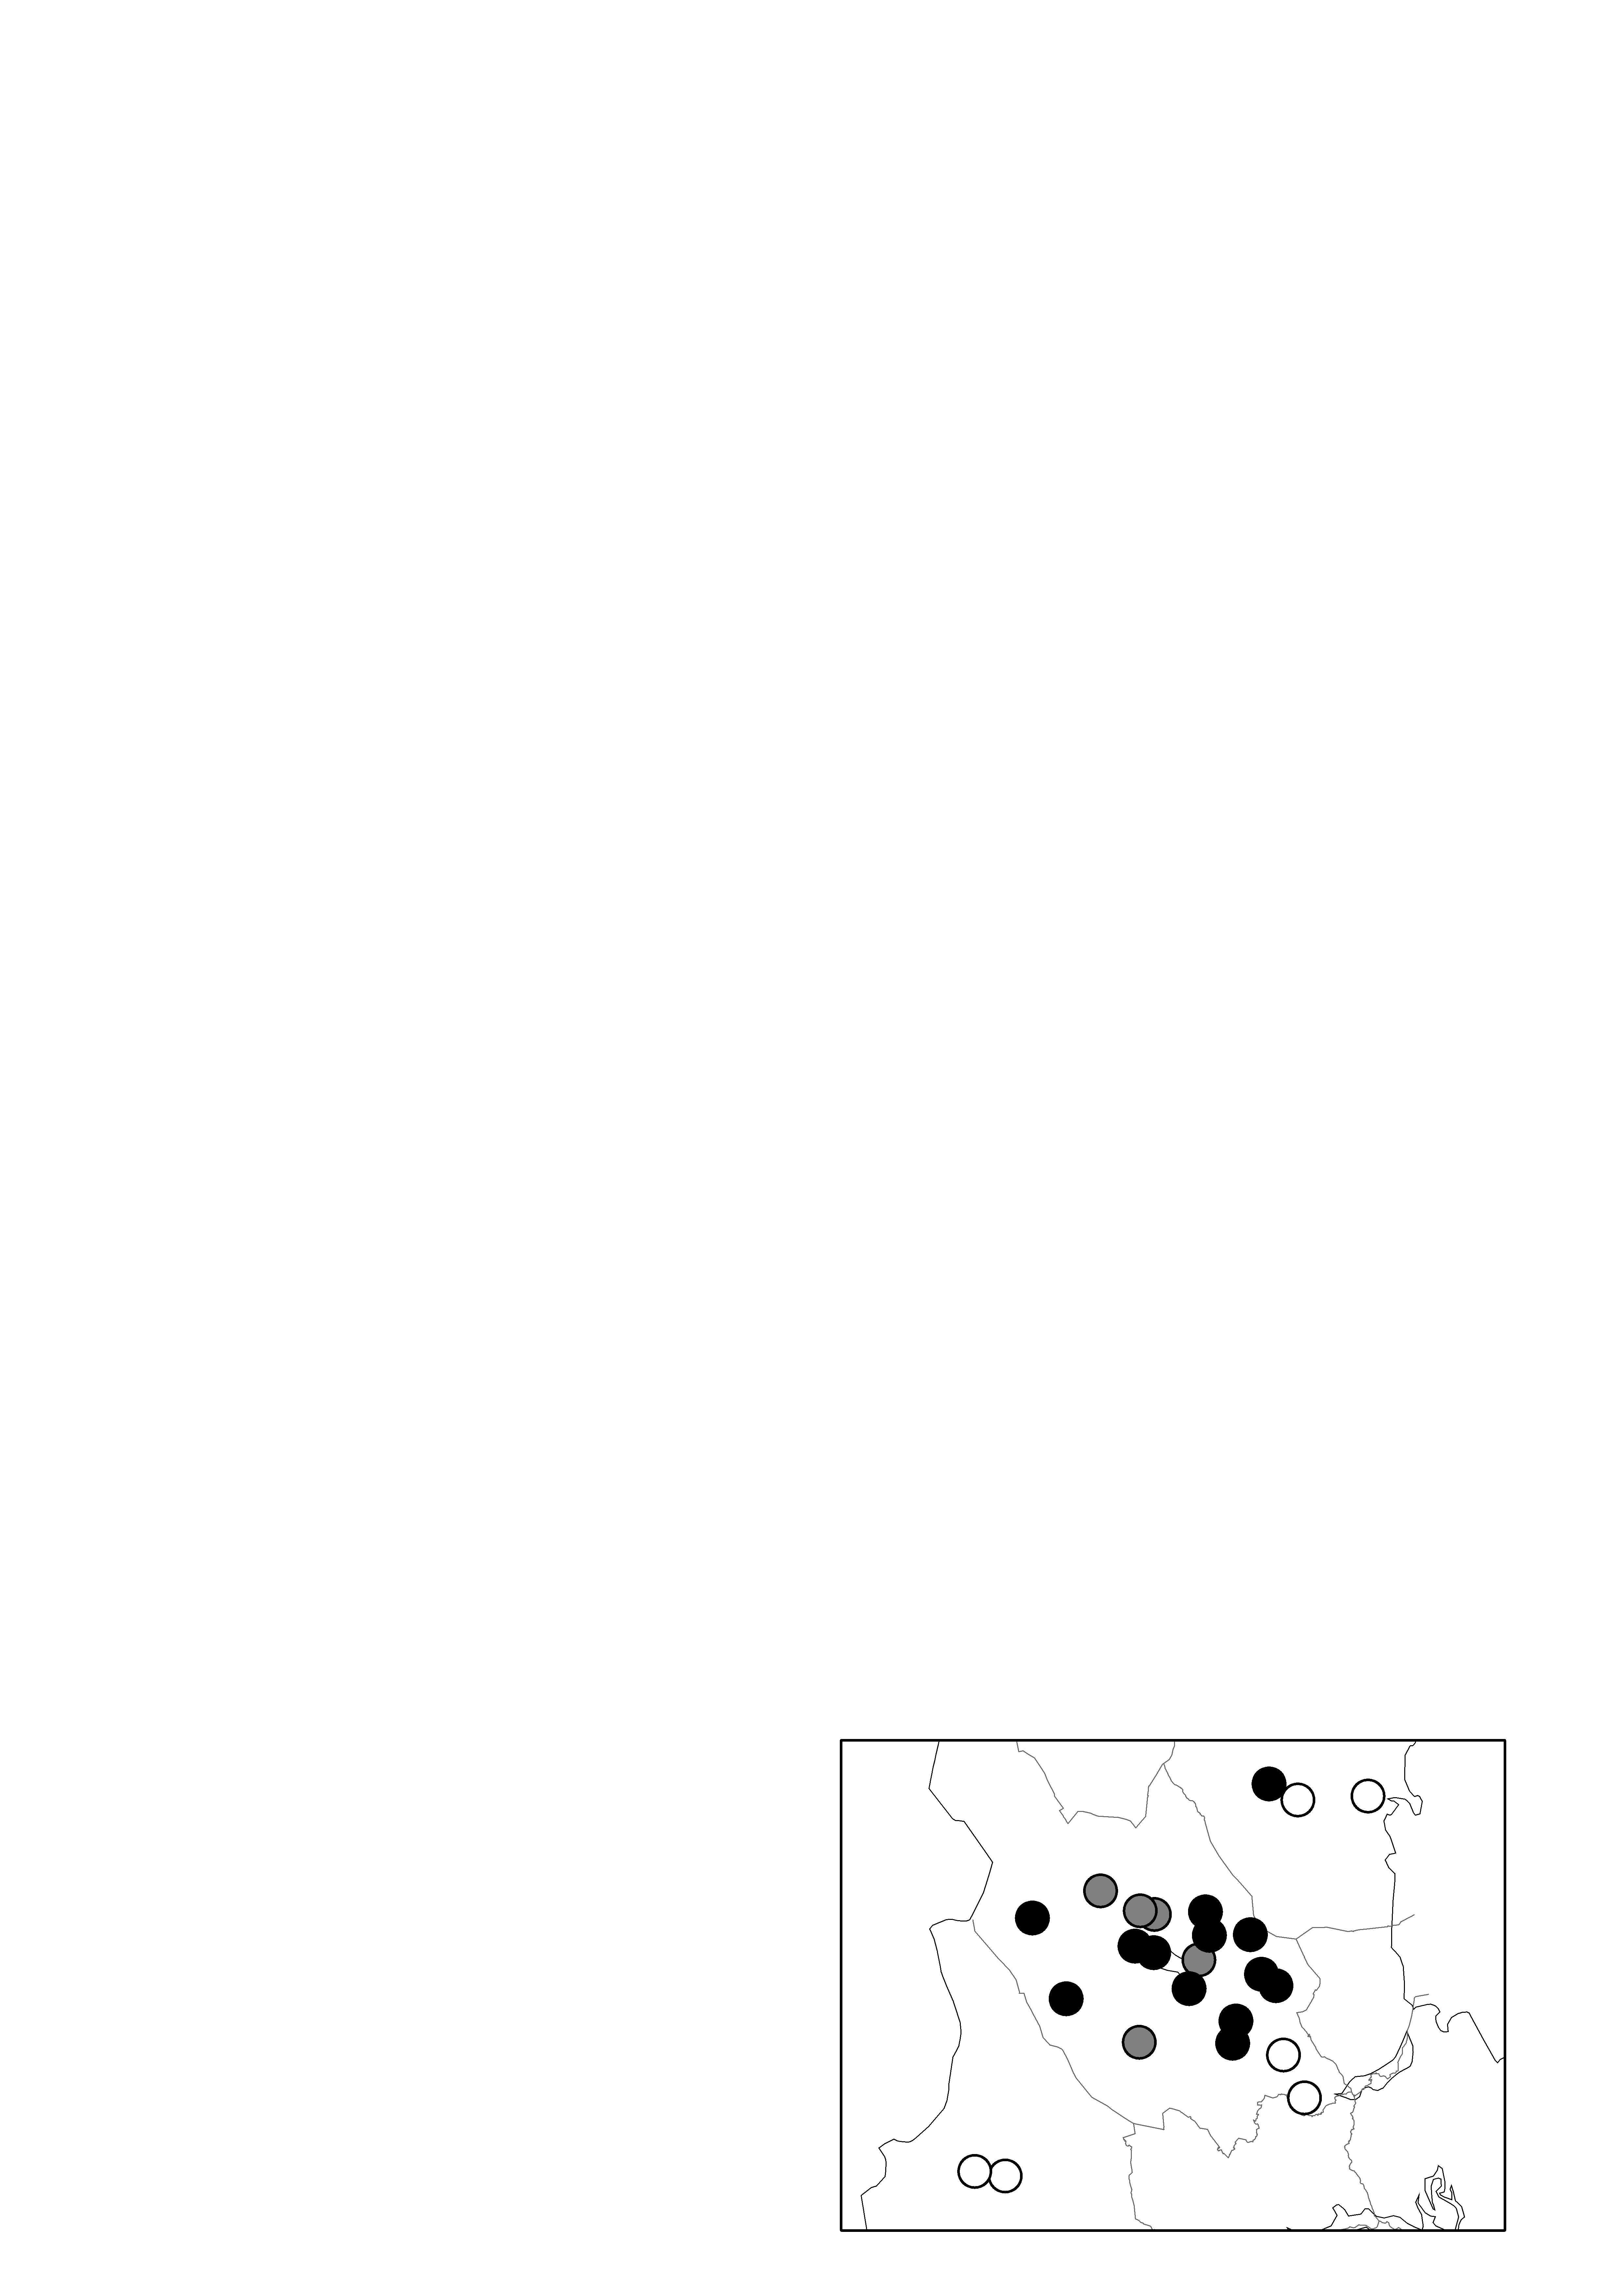
\includegraphics[height=.3\textheight]{figures/21_OccurrencesAbsPosCatCorpus}
\caption{Occurrences of absolute positives in the Cat Corpus. Black circles: absolute positives with apocope; grey circles: absolute positives without apocope; white circles: no absolute positives attested.}
\label{map:17}

\end{figure}